\documentclass{article}
\usepackage[utf8]{inputenc}

\title{Bohr's theory of hydrogen atom and Hydrogen Spectra}
\author{Jenni zhen }
\date{January 2016}

\usepackage{graphicx}

\begin{document}

\maketitle

\section{Introduction}
  In this paper, I am going o talk about Bohr's Theory of Hydrogen Atom and Hydrogen Spectra. In Bohr's Theory of Hydrogen Atom including derive Bohr's theory of the electron, using the theory of explain the observed spectra of emitted light of excited Hydrogen. Including all relevant constants and formula.
  
  
\section{Bohr's Theory of Hydrogen Atom}  
  Niels Bohr managed to explain the spectrum of atomic hydrogen by an extension of Rutherford's description of the atom. In that model, the negatively charged electrons revolve about the positively charged atomic nucleus because of the attractive electrostatic force according to Coulomb's law.

  Bohr model introduced by Niels Bohr depicts the atom as a small, positively charged nucleus surrounded by electrons that travel in circular orbits around the nucleus, but with attraction provided by electrostatic forces rather than gravity.He suggested that electrons could only have certain classical motions:

  Electrons in atoms orbit the nucleus.
  The electrons can only orbit stably, without radiating, in certain orbits at a certain discrete set of distances from the nucleus. These orbits are associated with definite energies and are also called energy shells or energy levels. In these orbits, the electron's acceleration does not result in radiation and energy loss as required by classical electromagnetic. The Bohr model of an atom was based upon Planck's quantum theory of radiation.

  
  $$ \Delta E=E2-E1=h\times v $$
  $$ V=\frac{1}{T}$$
  $$ L=n*\frac {h}{2\pi}=n*\hbar$$
  $$ n\lambda={2}{\pi}{r}$$
x
\begin{figure}[h!]
\centering
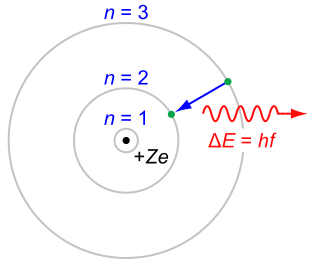
\includegraphics{1.png}
\caption{Bohr model}
\label{fig:Bohr model}
\end{figure}

\section{Hydrogen atom}
A hydrogen atom is an atom of the chemical element hydrogen. The electrically neutral atom contains a single positively charged proton and a single negatively charged electron bound to the nucleus by the Coulomb force. 


Niels Bohr obtained the energy levels and spectral frequencies of the hydrogen atom after making a number of simplifying assumptions in order to account for the failed Classical model. The assumptions included:

Electrons can only be in certain, discrete orbitals, thereby having a discrete radius and energy.
Electrons do not emit radiation while in one of these stationary states.
An electron can gain or lose energy by jumping from one discrete orbital to another.
The assumption that angular momentum was quantized can be expressed as:

$$L=n\times \hbar$$
$$rmeV=\frac{n\hbar}{r}$$
$$me^2V^2=\frac{n^2\hbar^2}{r^2}$$
$$\frac{mev^2}{2}=\frac{n^2\hbar^2}{2mer^2}$$
$$r=n^2a$$

As $$En=\frac{-e^2kE}{2rn}=\frac{1}{n^2}(\frac{-e^4kE^2me}{2\hbar^2})$$
   $$E1=-2.18 \times10^{-18} J$$
   $$En=\frac{E1}{n^2}$$


Bohr's second hypothesis combined with Planck's formula for quantized energy (E = hf) will now allow me to derive Balmer's equation.
$$ \Delta E=Em-En=\frac{E1}{m^2}-\frac{E1}{n^2}=E1(\frac{1}{m^2}-\frac{1}{n^2})$$
$$ \lambda=\frac{hc}{E}$$
$$ \lambda=\frac{hc}{E1(\frac{1}{m^2}-\frac{1}{n^2})}$$

\section{Lyman series}

 Lyman series is a hydrogen spectral series of transitions and resulting ultraviolet emission lines of the hydrogen atom as an electron goes from n more or equalto 2 to n = 1 (where n is the principal quantum number) the lowest energy level of the electron.
\section{Data}
\begin{table}[htbp]
\begin{center}
\footnotesize
\begin{tabular}{lcc}
\toprule
          $ transition &      \lambda nm\\                                                      
\midrule
  
 & $n=2\rightarrow n=1$\   &   121nm   \\
 & $n=3\rightarrow n=1$\   &   102nm  \\
 & $n=4\rightarrow n=1$   & 97.1nm  \\
 & $n=\infty\rightarrow n=1$   & 91nm  \\   
\bottomrule
\end{tabular}
\end{center}
  \caption{Lyman series}
  \label{tab:font-sizes}
\end{table}

  $$\frac{91nm}{(\frac{1}{1^2}-\frac{1}{2^2})}=121nm $$
  $$\frac{91nm}{(\frac{1}{1^2}-\frac{1}{3^2})}=102nm $$
  $$\frac{91nm}{(\frac{1}{1^2}-\frac{1}{4^2})}=97.1nm $$
  
 \begin{figure}[h!]
\centering
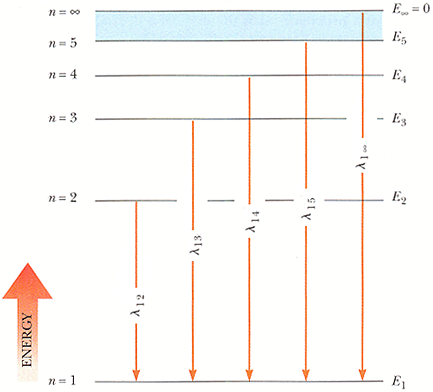
\includegraphics[scale=1]{3.png}
\caption{Lyman series}
\label{fig:univerise}
\end{figure}

 
  
\section{Balmer series}
The Balmer series or Balmer lines in atomic physics, is the designation of one of a set of six named series describing the spectral line emissions of the hydrogen atom.

\section{Data}
\begin{table}[htbp]
\begin{center}
\footnotesize
\begin{tabular}{lcc}
\toprule
          $ transition &      \lambda nm\\                                                      
\midrule
  
 & $n=3\rightarrow n=2$\   &   655nm   \\
 & $n=4\rightarrow n=2$\   &   485nm  \\
 & $n=5\rightarrow n=2$   &    433nm  \\
 & $n=\infty\rightarrow n=2$   & 364nm  \\   

\bottomrule
\end{tabular}
\end{center}
  \caption{Balmer series}
  \label{tab:font-sizes}
\end{table}

  $$\frac{91nm}{(\frac{1}{2^2}-\frac{1}{3^2})}=655nm $$
  $$\frac{91nm}{(\frac{1}{2^2}-\frac{1}{4^2})}=485nm $$
  $$\frac{91nm}{(\frac{1}{2^2}-\frac{1}{5^2})}=433nm $$
  
\begin{figure}[h!]
\centering
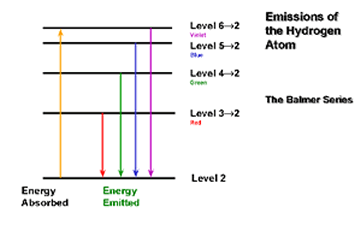
\includegraphics[scale=1]{balmer2.png}
\caption{Balmer series}
\label{fig:univerise}
\end{figure}



\end{document}
